\section{Expected System Diagram}
\begin{figure}[!ht]
    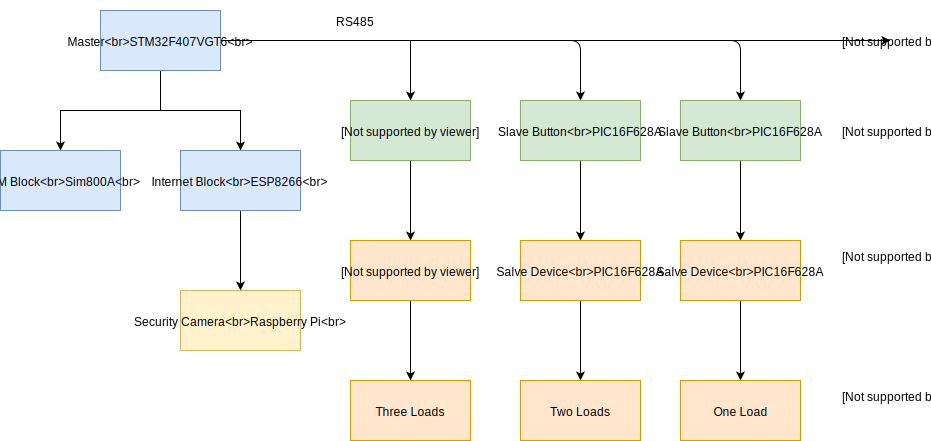
\includegraphics[scale=0.5]{images/hardwareBlock.png}
    \caption{Expected hardware blocks}
    \label{fig:hardwareBlock}
\end{figure}

    \begin{table}[h!]
    \begin{center}
    \begin{tabular}{ |c||c||c|  }
      \hline
      Attributes & Detail & Notes\\
      \hline
      Maximum number of devices&   99& Can be extended by\\
      & &extending command frame\\
      \hline
      Longest distance supported&   1200 meters&\\
      \hline
      Communication method &Mainly RS-485&\\
      \hline
      Wi-Fi connection & Wi-fi 2.4GHz&\\
      \hline
     \end{tabular}
     \caption{System ideal characteristics}
     \label{table:idealCharacteristics}
    \end{center}
    \end{table}
    In Figure~\ref{fig:hardwareBlock}, there are blocks named Master, Slave Buttons, Slave Devices, GSM block, Internet block and Security Camera. Each block is indicated with implemented hardware and how they connect to each other. As in the figure~\ref{fig:hardwareBlock}, Master is connecting with number of Slaves by UART over RS-485; Also, Master is implemented with GSM and Internet blocks in order to help end user controlling devices and receiving alerts over GSM or Wi-Fi. Each slave connects to the system has the same working principle but different names. In this thesis, there are two slave-2-devices and one slave-3-devices alongside with two slave-2-buttons and one slave-3-buttons to control the loads, respectively. Besides, the author designed one slave-2-buttons and one slave-1-button to control three out of seven existed devices. Three slave-devices are implemented with relays switch state for devices in the house, last device (Device 3) of slave-3-devices is assigned as the Main Door trigger to demonstrate the Security Camera System with Facial Recognition later on.

    Internet Block is the middle man for communicating between Application Server and the System. With this block implemented, end-user can control devices without pushing the physical buttons, which may causes difficulties for users because the owners can control their house whenever and wherever they want. Besides, with the help of the Application Server, end-users can collect and monitor data in the house in order to diagnostic and maintain precisely. GSM block should be installed in order to help in the event that Internet block is having unexpected problems.

    Security Camera block is the block that monitors the main door and inside the house. The camera installed outdoor is responsible for outdoor security in which it will track people entering the house with a facial recognition system. Additionally, indoor camera should handle the motion detection system while the owner is not at home in order to find strange motion which maybe a burglar breaking in the house. These two system will track and alert by emails, mobile application and text message over GSM network in the case that they detect something. Furthermore, the three-dots indicates that the system can be extended with number of slaves over RS-485, but only up to 99 dues to the limitation of command frame.
%Master hardware design
\section{Master}
    \subsection{Microcontroller Requirements}
    There are few requirements for the Microcontroller that the author decided to build the system for the thesis, listed as following.
    \begin{itemize}
        \item Support UART in order to communicate with other modules, namely RS-485, ESP8266 and SIM800A.
        \item Has widely support community.
        \item Easy to learn to program.
        \item Extendable with installed components.
        \item Price and ability for effortless replacement.
      \end{itemize}
      \begin{figure}[!ht]
        \begin{center}
        \includegraphics[scale=1]{images/stm32f4_discovery.jpg}
        \caption{STM32F4 Discovery Kit}
        \label{fig:stm32Kit}
        \end{center}
      \end{figure}
      Based on the requirements, the chosen MCU is STM32F407VGT6 with STM32F4 Discovery Kit from STMicroelectronics. Figure~\ref{fig:stm32Kit} refers the real kit in the market. It is considered as a suitable MCU because of the following reasons.
      \begin{itemize}
        \item The board has large support community.
        \item Programmed with C language with countless documents.
        \item MCU used is STM32F407VGT6, with core ARM Cortex 32bit M4, clock up to 168Mhz.
        \item Support up to 140 I/O.
        \item Flash memory 1MB.
        \item Easy to flash even with end-user.
        \item Cheap price and easy to find replacement parts.
      \end{itemize}
      \begin{figure}[!ht]
        \begin{center}
        \includegraphics{images/headerMcu.PNG}
        \caption{Header for STM32F4 Discovery Kit}
        \label{fig:headerMcu}
        \end{center}
      \end{figure}
      In this thesis, to ensure the effortless replacement of the system parts, the author designed with modules attached on PCB by using headers. With this method, whenever an error occurs to any part of the system, end-user can replace the broken part easily without replacing the whole system. Figure~\ref{fig:headerMcu} shows the headers on Master board for STM32F4 Discovery Kit which is chosen for the thesis. In addition, it shows the connection pin of the MCU with other modules over UART. To be more specific, MCU connects with RS-485 module over UART1 via pin PB6-PB7, with module ESP8266 over UART2 via pin PD5-PD6, with module SIM800A over UART3 via pin PD8-PD9.
      %hardware RS-485
      \subsection{Module RS-485}
      \begin{figure}[!ht]
        \begin{center}
        \includegraphics[scale=0.63]{images/header485.PNG}
        \caption{Header for module RS-485}
        \label{fig:header485}
        \end{center}
      \end{figure}
      \begin{figure}[!ht]
        \begin{center}
        \includegraphics[scale=1]{images/module-rs485.png}
        \caption{Module RS-485}
        \label{fig:module485}
        \end{center}
      \end{figure}

      Figure~\ref{fig:module485} refers the cheap version of module TTL to RS-485 on the market. It integrated IC MAX485 as the main component and other sub-components included termination resistor. This module is stable enough for the system and easy to replace due to its cheap price but does has a weakness which is if it is broken, end-user cannot know unless further tests on the module is processed. The table~\ref{table:module485PinOut} indicates the pin out guideline to connect with the MCU. According to datasheet of IC MAX485, RE and DE must be connected for the MCU to control the module based on logic level, in which the module is transmitting if the pins are pull up to 1, otherwise it is receiving.
      \begin{table}[h!]
        \begin{center}
        \begin{tabular}{ |c||c|  }
          \hline
          Pin & Detail\\
          \hline
          VCC& 5V\\
          \hline
          A&   Non-inverting Receiver Input and Non-inverting Driver Output\\
          \hline
          B &.Inverting Receiver Input and Inverting Driver Output\\
          \hline
          GND & GND, should be 0V\\
          \hline
          RO & Receiver Output (to Rx pin of microcontroller)\\
          \hline
          RE & Receiver Output Enable (Low to enable)\\
          \hline
          DE & Driver Output Enable (high to enable)\\
          \hline
          DI & Driver Input (to Tx pin of microcontroller)\\
          \hline
         \end{tabular}
         \caption{Module UART TTL to RS-485 pin out}
         \label{table:module485PinOut}
        \end{center}
        \end{table}
      
      Figure~\ref{fig:header485} shows the headers which are used on Master board for RS-485 module in figure~\ref{fig:module485} and the headers of RJ-11 female jack for RS-485 output of the Master. The reason for choosing RJ-11 jack and its compatible cable is the cable suits for the project which needs four wires, in which two are the signal wires (A and B of RS-485 standard) and the other two are the pair providing power for other slaves (12V and GND). With this method, a four-wire twisted cable with shield is used in order to keep the noise as low as possible and still, provides the power along the whole system with only one cable connected.

      \subsection{Module ESP-8266}
      This module is implemented to establish the connection between the Application Server and the System. End-users can control and monitor their system with a website or an android application over Wi-Fi connection with module ESP-8266. There are various versions of module using ESP-8266 on the market, but the full name of the chosen module is ESP-8266 NodeMCU lua CP2102. It is a small size kit that integrated with ESP8266 SoC, other components and it is also compatible with Arduino IDE which makes it become the easiest to use ESP-8266 module in comparison to other versions.
      \begin{table}[h!]
        \begin{center}
        \begin{tabular}{ |c||c|  }
          \hline
          Attribute & Detail\\
          \hline
          SoC& ESP8266 Wifi SoC\\
          \hline
          Firmware&   NodeMCU Lua\\
          \hline
          Flash chip &CP2102\\
          \hline
          GPIO & compatible with firmware of Node MCU\\
          \hline
          Power supply & 5V DC with Micro USB or Vin\\
          \hline
          GPIO logic level & 3.3V\\
          \hline
          Integrated LED & Reset, Flash and Status indicator\\
          \hline
          Dimension & 25mm x 50mm\\
          \hline
          Others& Compatible with Arduino IDE\\
          \hline
         \end{tabular}
         \caption{Module ESP-8266 NodeMCU lua CP2102 remarkable characteristics}
         \label{table:moduleEspDetail}
        \end{center}
        \end{table}

        \begin{figure}[!ht]
            \begin{center}
            \includegraphics[scale=0.9]{images/module-esp.png}
            \caption{Module ESP-8266 NodeMCU lua CP2102}
            \label{fig:moduleEsp}
            \end{center}
          \end{figure}

          \subsection{Module SIM800A}
          %TODO: finish module SIM800A

          \subsection{Power for Master}


